http://wwwcompass.cern.ch/

HPS Hall B: https://arxiv.org/pdf/1505.02025.pdf

CLAS12
How thick is CLAS12 target? Calculate out luminosity
at small t expect to see a cos(2phi) dependence, large t cos(phi) dependence
Calculate e-p scattering kinematics and compare to results from analysis
How many DVMP measurements have been made? What is shitty about them and why? What can CLAS do better / differently? Large acceptance --? Not in right range? High data rate. Hall A low kinematic coverage. What is the t resolution? Q2 resolution? 
CLAS12 – how many electrons per second? Per bunch? 

No proton – don’t need it, but should have it as it gives u s better defined final state, nail this process down, want to have a really clean process, its already hard. CLAS12 is great because of its huge kinematic coverage. If you want high luminosity as a specific regime ok maybe go to Hall, A, but that’s something else.

What triggers CLAS12 event time?
How does pion - kaon separation in LTCC work?

work out, giving FTOF timing resolution, and distance, what energy PID works up to
Also remind self of functional form of Beta vs P curve
Energy range of electrons, protons, pions (gammas) in DVMP events

Read nature paper – extract EMT energy momentum tensor




rough idea of cross section - nanobarn?


How are events mapped back to one collision bunch? And how many electrons are in each bunch?
    We can work this out - how long does it take in e.g. 5038 to accumulate 100 million events? How many electrons does that correspond to? What luminosity does that correspond to? How many ep events are recorded in 5038? How many DVMP events did you record? BTW, what data size did CLAS work off of?
    
    
    How many photons convert on way to pcal at CLAS12?




In the end this will need to be repeated for all xb, q2 bins. Why are we doing this? IDK, right now. But I’m fixin to find out! (plotting structure functions) Like what is it that we want at the end?


Jlab nuclear femtography: https://www.youtube.com/watch?v=JMP5Gh62gHQ

Relation between Compton form factors (or generalized form factors) DVMP and GPDs?

what are problems with your / other detectors?
Why not look for longitudinal spatial ditributions? Because this direction is contracted by a factor of proton radius / gamma, where gamma – 10 GeV/ 0.5 MeV = 20,000  longitudinal distance is 0.5 fm * 10^-4 = 0.05 am = 50 zeptometers across – it is “pancaked”
What Q2 and X and W range can I probe?

winger and GTMDs are related by a fourier transform from the Detla variable to the transverse spatial variable? The delta variable is

\section{GlueX}
    \indent Gluex looks into studying the spectrum of hybrid and exotic mesons to test QCD. None have been definitively identified. Uses photoproduction to produce mesonic states, using linearly polarized photons, which allows for the analysis of certain polarization observables taht are thought to make identification of exotic states feasible. Search and study exotic hybrid mesons. Photoproduction is expected to be particualry effective in producing and identifying these states. Also pursues conventional meson spectroscopy. Partial wave analysis allows for the reconstruction of all the intermediate states, allowing for the extraction of their quantum states (J P and C). 



Hall B stuff:
http://faculty.fiu.edu/~baraue/research/moeller/p2.html

Hall A also uses a Moller polarimeter:
https://hallaweb.jlab.org/equipment/moller/

As does Hall C:
https://www.jlab.org/physics/hall-c/moller

The Hall-C Moller Polarimeter measures the polarization of the electron beam arriving in Hall-C. It does so by observing the rate of production of Moller electrons at 90 degrees in the center of mass when the beam strikes a thin iron target. The outer shell electrons in the iron are polarized parallel (or anti-parallel) to the beam direction by a 4 Tesla magnetic field. The Moller electron production rate differs when the beam and target electron spins are aligned parallel or anti-parallel to one-another. Measurement of this rate difference provides a measure of the beam polarization.

The Hall-C device is designed to provide an absolute polarization measurement with accuracy better than 0.5\%. A system of movable collimators and a pair of quadrupole magnets allows the system to be tuned to operate at any beam momentum between about 0.9 and 6 GeV/c. The figure below shows the layout of the Polarimeter, which is placed in the beam alcove upstream of Hall-C.




What is JLab hadron spectroscopy at Jlab

JLab data rate in inverse femtobarns?
How far from target is FTOF?


Hi Bobby, so sorry for late reply I was busy with readiness review preparation.So Q2>1 is indeed for deeply virtual events, however it has no relation with lepton/hadron angle. There are pi0 events in the region below 1GeV2, and they are also pi0 events. The limit on 1GeV2 is somewhat artificial. Ideally we are looking at the asymptotic freedom, so Q2 should be infinity, but we are hoping that 1GeV2 is big enough to apply models that are based on asymptotic freedom. There are many terms also that are proportional to powers of t/Q2. So we need reasonably big Q2 to apply GPDs models. And in fact CLAS kinematics is often questioned to be too small for GPDs theoretical models.Anyway, inbending CLAS12 data by default don't have any low Q2 data because of the electron acceptance. If you see lower Q2 they might come from outbending data, and then indeed you would need to implement hardcoded cut on Q2. But if it's the same runs, just different cooks, then it's strange, and we should investigate it further.






What is meant by chiral phase transition - The chiral phase transition is between "chiral condensate=0" and "chiral condensate != 0". And the connection between chiral phase transition and confinement transition is shown in Fig 12.2 in this book (I already upload to NuPAX Part 3):

Factorization theorem of DVCS


http://www.scholarpedia.org/article/Axial_anomaly

Regge theory: in quantum physics, Regge theory (/ˈrɛdʒeɪ/) is the study of the analytic properties of scattering as a function of angular momentum, where the angular momentum is not restricted to be an integer multiple of ħ but is allowed to take any complex value. he nonrelativistic theory was developed by Tullio Regge in 1959. A regge trajectory is a path in the complex angular momentum plane describing evolution when solving potentials (such as Coubomb or Yukawa) with complex values allowed. The main result of the theory is that the scattering amplitude for potential scattering grows as a function of the cosine {\displaystyle z}z of the scattering angle as a power that changes as the scattering energy changes. This, combined with S-matrix theory, form the basis for string theories. Shortly afterwards, Stanley Mandelstam noted that in relativity the purely formal limit of {\displaystyle z}z large is near to a physical limit — the limit of large {\displaystyle t}t

How do cosmic Ray's get accelerated
Look up tensor force of meson exchange



Be able to draw the detector system REALLY Well
Be able to describe all (at least 3) detectors in extreme detail 
All analysis assumes factorization, is it reasonable to assume this? Is there a way to test this?

What is the kinemeatic range accessible to the experiment?
What is the point of doing this at CLAS12 as opposed to anywhere else

What is meaning of the kinematic variable xi, physically?


Other note – wigner distributions just practically not worth trying to get at any point in the near future
Other physics that can be tested by measuring pion cross section? Such as test factorization? 
overall importance of this? – a lot more kinematic data points, way bigger than the 3 from the pressure of the proton paper from volker and latifa, and that got a ton of attention

DIS – 1D image of proton, longitudinal momentum, no longitudinal spatial because everything pancakes.
Do not NEED to measure all final state particles (e.g. Hall A did not need to do this) but adds much redundancy which helps discern from background a lot – e.g. read the hall A papers! on dvcs and dvmp.
DVMP – 2-3D image of proton, GPDs, GCFF, etc.

Hall A – low kinematic coverage?

How many DVMP measurements have been made? Where does this research fit in with the field? 
How do you know you are in dis or dvcs regimes
How does CLAS12 trigger?
How do we get from gdps to form factors


weak isospin, qWeak
What are the physical intuitions of the 4 chiral even and 4 chiral odd GPDs
Memorize GTMD – TMD – PDF – Q – GPD cube

Understand the difference between a structure function and a PDF – how do we get PDFs from DIS? How do we get GPDs from DVMP?

proton spin problem

COMPASS – Hall A – CLAS6 – strengths and weaknesses of each? What is their t resolution? Q2 resolution? Kinmeatic range?

What is the twist expansion

Wigner distribution function

Why is clas12 / jlab important for the measurement / why can't you do it at other accelerators
What q2 range can I reach? and why?

Talking to Axel on 3/9/20
Research:
Memorize GTMD – TMD – PDF – Q – GPD cube
“We start with an EM probe because we can calculate out the hard perturbative part of the interaction (facotorization) and don’t know how to deal analytically with whats left, but we can group it into a GPD”. 
By measuring DVMP, we can get information about GPDs in the following way – in the leading twist approximation / some other formalism bullshit, dvmp cross section is described by the generalized Compton form factors, which themselves are (to leading twist etc.) convolutions of GPDs, so the dvmp cross section sets constraints on GPD behavior.
The way we can measure them is at CLAS12 at jlab --- enter detector talk.

NEED to expect questions on how many photons convert on route to the PCAL/ECal


HTCC – electron ID
LTCC – pion vs. kaon id
Now talk about Why CLAS12 / what this research will give you
COMPASS – Hall A – CLAS6 – strengths and weaknesses of each? What is their t resolution? Q2 resolution? Kinmeatic range?
How many DVMP measurements have been made? Where does this research fit in with the field? 
What is shitty about previous measurements and why? What can CLAS do better / differently? Something about large acceptance/ in the right kinematic range where approximations are valid, high data rate / luminosity, etc.
Hall A – low kinematic coverage?
Overall talk:
Motivation / background:
	DIS – 1D image of proton, longitudinal momentum, no longitudinal spatial because everything pancakes.
	DVMP – 2-3D image of proton, GPDs, GCFF, etc.
JLab / CLAS12
	Jlab layout / clas12 layout, experiment design
		NEED to expect questions on how many photons convert on route to the PCAL/ECal

Feedback on Or from what went wrong on the exam:
Where does what you’re doing fit in with the analysis of DVMP / DVCS
Where does this analysis fit in with the scope of what we know about proton structure?




        \begin{figure}[H]
            \centering
            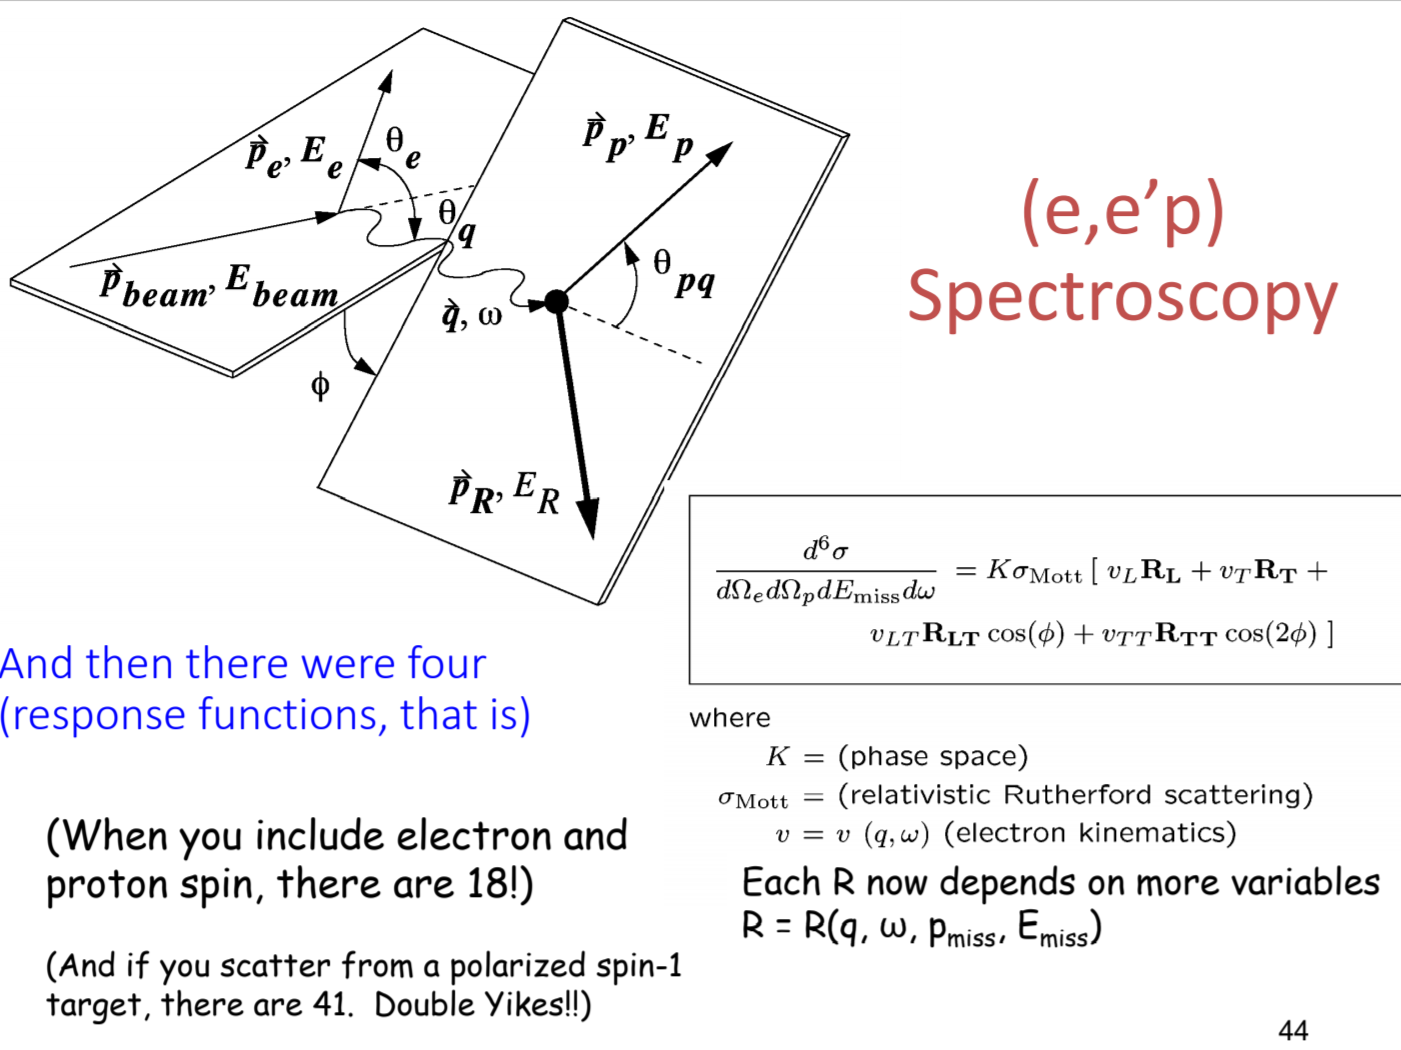
\includegraphics[width=10cm]{NuclearPhysics/modules/lepton-scattering/pics/response-funcs.PNG}
            \caption{Caption}
        \end{figure}
        
        
        
Need to read EIC paper, have an understanding of where EIC lives, and also take care of HERMES land - where does that data live

why cant we go to higher luminosity? (i.e. what is the factor limiting us from going to higher luminosities? I dont think it is triggr rate




Sigma L = sum of the structure functions initiated by a longitudinal virtual photon
Sigma T is the sum of structure functions which are initiated by a transverse virtual photon of positive and negative helicity with and without nucleon helicity flip

Sigma LT corresponds to interferences involving products of amplitudes for longiutidal and transverse photons

Sigma TT is an interference inoling products of transverse positive and negative photon helicity ampitidues.


Exclusivity cuts: 

missing mass squared of electron-proton sytem should be the mass squared of the pion ***work out these kinematics***

The missing energy of the e p pion system is zero

The gamma gamma invariant mass is the pion mass
  
            
            
            
            CLAS 2014 paper – asymptotic leading order handbag approach where sigma L is dominant is not applicable at present values of Q2

Cross section needs to be corrected for pion branching ratio (even tho its 99%), normalized to elastic cross section, radiative effects, acceptance, etc. 

            
            
            5 cm long target, 100inverse nanobarns per second. 300 mC of data taken. 6% of data taken, 80k DCS events found
            
            
            
“possibility to study GPDs in exclusive scattering processes rest s on factorization theorems, whicha are proven for DVCS and light meson production in the limit of Q^2 appraoching infinity

Factiorizion lets you treat one part of the interaction perturbately, while the nonperturbative reimatiner is embodied in the GPD. This means there is a reaction dependent part, and a reaction indpenendet part which contains the GPD. Only proven for asymptotoically large Q^2, but evidence suggests it works well even down to 1.5 GeV2 for DVCS, but current limits for DVMP are not clear. 

There are eight GPDs. Four correspond to parton helicity conserving (chiral even) processes, H, H~, E, and E~ and four corresponding to parton helicity flip (chiral odd) processes HT, HT~, ET, and ET~. 


CLAS kinematics: xb between 0.2 and 0.5, q2 between 1 and 4. 7 billion total events, 100,000 DVPP events. Integrated luminosity of 20 inverse femtobarns. Largest uncertainties were absolute normalization ~ 5%, and proton id ~ 3%. Overall uncertainty is about 10%. 


Very briefly, this research is  studying the 3D structure of the proton by measuring the cross section for a specific ep scattering channel. This channel - deeply virtual pion production - has a cross section which is described by generalized parton distributions, which map out the proton in terms of longitudinal momentum and transverse spatial distributions of quarks. 

  Gamma energies and angles, protons,electrons  

            
            

sigma_L scales as 1/Q^6, sigma_T scales as 1/Q^8


“factorization proved for longitudinally polarized quarks, assumed to hold for DVMP but there is question if it actually holds at JLab, so that is soemthign we are looking into. If it does hold, then sigma_T will be small, and the GK model will be applicable?

DVpiP x-section ~ few to hundreds of nanobarns, pp inclusive ~ millibarns, elastic ~ barns (at low Q2)
electrons drift 5 cm/microsecond in Argon, normal drift times in Drift chambers of 1 or 2 microseconds. 

Hall A momentum resolution - 10^-4, 3\% uncertaintiy in cross section measurment, able to really constrain exclusibity from missing momentum even though they dont have the proton. CLAS12 annot do this since our resolution is nowhere near as good - we are at level of 1 to 10 percent resolution, not 0.01 percent

CLAS12 is very good PID at CLAS12, good high quality data, allows us to start at valence quarks where things are better known, very precise data which will enivatbily inform us about GPDs. , since in valence quark regime can compare to data such as PDFs. Its important to have the data, you can interpret it how you like. Really after the tomography of the proton


What is the intuation for the longitudinal polarization of the photon (epsilon) being a function of kinematic variables in the way that it is? What is the physical significance? 


luminsotiy limited by BST and DC – if we increase the luminosity, the detector occupancies will get too high and the resolution will suffer - per Mauri, May 2020